\chapter{Théorie du risque}

\section{Processus Stochastique}

\subsection{Processus Homogène Composée}

\paragraph{Definition}
\[ S(t) = \sum_{k=1}^{N(t)} X_k \]

\paragraph{Fonction de répartition}
\[ F_{S(t)}(x) = \prob{N(t) = 0} + \sum_{k=1}^\infty \prob{N(t) = k} * F_{X_1+...+X_k}(x) \]
\begin{lstlisting}[language=R, caption={Exemple Pois-Gamma}]
F_s <- function(x, t){
    dpois(0, lambda * t) + sum(sapply(1:k0, function(k) dpois(k, lambda * t) * pgamma(x, alpha * k, beta)
}
\end{lstlisting}

\paragraph{Value at risk}
\[ \VaR{S(t)} = F_{S(t)}^{-1}(k) \]

\begin{lstlisting}[language=R, caption={Exemple Pois-Gamma}]
VaR_s <- function(kappa, t){
    if(kappa <= dpois(0, lambda * t)
        return(0)
    uniroot(function(x) F_s(x, t) - kappa, c(0, 10000))$root
}
\end{lstlisting}

\paragraph{Tail Values at Risk}
\[ \TVaR{S(t)} = \sum_{k=0}^\infty \prob{N(t) = k} \cdot \TVaR{X_1+...+X_k}\]

\begin{lstlisting}[language=R, caption={Exemple Pois-Gamma}]
TvaR_S <- function(kappa, t){
    sum(sapply(1:k0, function(k) dpois(k, 1.8 * t) * alp    ha * k / beta * (1 - pgamma(VaR_s(kappa, t), (alpha*k)+1, beta)))) / (1 - kappa)
}
\end{lstlisting}

\subsection{Processus Poisson Mixte}

\paragraph{Definition}
Soit $\Lambda$ une variable aléatoire positive (continue ou discrète). Si le
processus de comptage $\underline{N} = \{N(t);t \geq 0\}$ étant donné que $\Lambda = \lambda$ est
un processus de Poisson de taux $\Lambda$ alors $\underline{N} = \{N(t);t \geq 0\}$ est appelé
un processus de Poisson mixte.  \\ 

Les accroissements du processus de Poisson mixte $\underline{N}$ sont \textbf{indépendant} et \textbf{stationnaire}. \\
\paragraph{Preuve (stationnaire)}
    \begin{align*}
        M_{N(t, t+s]}(r) &= \esp{e^{r N(t, t+s}} \\
                         &= \esp[\Lambda]{\esp{e^{r N(t, t+s]}|\Lambda}} \\
                         &= \esp[\Lambda]{e^{\Lambda t(e^r - 1)}} \\
                         &= M_\Lambda(t(e^r - 1)) \\
                         &= M_{N(t)}(r) \\
                         &= \text{Stationnaire car fonction de $t$ seulement}
    \end{align*}

\paragraph{Preuve (indépendance)}
A faire

\begin{note}
    Les temps-inter siniste sont échangeable, mais ne sont pas indépendant. Par contre,
    les temps-inter siniste $(W_1|\Lambda)$ et $(W_2|\Lambda)$ sont conditionnelement indépendant et $(w|\Lambda) \sim \text{Exp}(\lambda)$. \\
\end{note}

\begin{figure}[!ht]
    \centering
    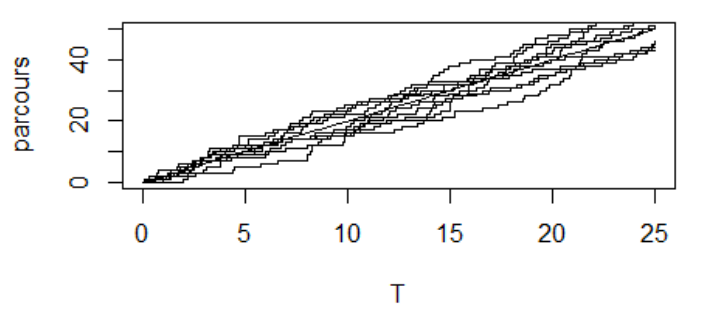
\includegraphics[scale=0.5]{src/TheorieDuRisque/SimulationProcessusPoisson.png}
    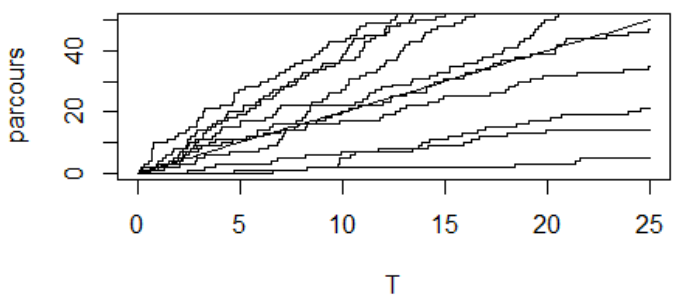
\includegraphics[scale=0.5]{src/TheorieDuRisque/SimulationProcessusPoissonMixte.png}
    \caption{Comparaison entre un processus de Poisson homogène et un processus de poisson mixte. Le graphique du bas représente le processus mixte.}
\end{figure}

\begin{align*}
    \prob{N(t) = n} &= \int_{-\infty}^\infty \prob{N(t) = n | \Lambda} \cdot f_\Lambda(\lambda)\: d\lambda \\ 
    &\text{si } \Lambda \sim \Gamma(\alpha, \beta) \\
    &= \frac{\Gamma(\alpha+n)}{\Gamma(\alpha)k!} \left( \frac{\beta}{\beta + t} \right)^\alpha \left( \frac{1}{\beta + t} \right)^n \sim \text{BinNeg}(\alpha, \frac{\beta}{\beta + t})
\\
    \prob{N(t, t+s] = n} &= \int_{-\infty}^\infty \prob{N(t, t+s] = n | \Lambda} \cdot f_\Lambda(\lambda)\: d\lambda \\
    &= \int_{-\infty}^\infty \prob{N(s) = n | \Lambda} \cdot f_\Lambda(\lambda)\: d\lambda 
\\ \\
    \prob{N(t) = k_1, N(t, t+s] = k_2} &= \int_{-\infty}^\infty \prob{N(t) = k_1, N(t, t+s] = k_2| \Lambda} \cdot f_\Lambda(\lambda)\: d\lambda \\
    &= \int_{-\infty}^\infty \prob{N(t) = k_1 | \Lambda} \prob{N(s) = k_2 | \Lambda}\cdot f_\Lambda(\lambda)\: d\lambda
\end{align*}
\begin{align*}
    \esp{N(t+s)|N(t) = k_1} &= \esp{N(t) + N(t, t+s] | N(t) = k_1} \\
    &= k_1 + \esp[\Lambda]{\esp{N(t, t+s]|N(t) = k_1, \Lambda}|N(t) = k_1} \\
    &= k_1 + \esp[\Lambda]{\lambda t|N(t) = k_1} \\
    &= k_1 + \int_{-\infty}^\infty \lambda t \frac{f_{\Lambda, N(t)}(\lambda, k_1)}{\prob{N(t) = k_1}}\: d\lambda \\
    &= k_1 + \frac{\int_{-\infty}^\infty\lambda t \prob{N(t) = k_1|\Lambda} f_\Lambda(\lambda)\:d\lambda}{\int_{-\infty}^\infty \prob{N(t) = k_1|\Lambda} f_\Lambda(\lambda)\:d\lambda} \\
    &\text{si } \Lambda \sim \Gamma(\alpha, \beta) \\
    &= k_1 + \frac{\alpha + n}{\beta + t}
\end{align*}
\begin{align*}
    F_{W_1}(t) &= \int_{-\infty}^\infty F_{w_1|\Lambda}(t) f_\Lambda(\lambda)\,d\lambda \\
    &\text{si } \Lambda \sim \Gamma(\alpha, \beta) \\
    &= \left( \frac{\beta}{\beta + t} \right)^\alpha \sim \text{Pareto}(\alpha, \beta)
\\ \\
    F_{W_1, W_2}(t_1, t_2) &= \int_{-\infty}^\infty F_{W_1}(t_1) F_{W_2}(t_2) f_\Lambda(\lambda)\,d\lambda\\
    &\text{si } \Lambda \sim \Gamma(\alpha, \beta) \\
    &= \left( \frac{\beta}{\beta + t_1 + t_2 } \right)^\alpha \sim \text{Pareto Mulivarié}
\end{align*}
